\chapter{Semi-Statistical Study of Dimming-CME Relationship}
\label{chapterstatistical}

% Mini-abstract
Extreme ultraviolet (EUV) coronal dimmings are often observed in response to solar eruptive events. These phenomena can be generated via several different physical processes (see Chapter \ref{chaptermechanisms}). For space weather, the most important of these is the temporary void left behind by a coronal mass ejection (CME). Massive, fast CMEs tend to leave behind a darker void that also usually corresponds to minimum irradiance for the cooler coronal emissions. If the dimming is associated with a solar flare, as is often the case, the flare component of the dimming in the cooler coronal emission can be isolated and removed from the dimming light curve using simultaneous measurements of warmer coronal lines (see Chapter \ref{chaptercasestudy}). In the present Chapter, we apply this technique to 38 dimming events: the two case studies from Chapter \ref{chaptercasestudy} plus 36 additional events taken from two separate two-week periods in 2011. Dimming is then parameterized in terms of depth and slope for each of the events. We provide statistics on which combination of wavelengths worked best for the correction method, describe the fitting methods applied to the dimming light curves, and compare the dimming parameters with corresponding CME parameters of mass and speed. The best linear relationships found with an accuracy of about 20\% are that the CME speed is about $630 km\ s^{-1}$ times the dimming slope ($\%\ hour^{-1}$) and the CME mass is about $1.03 \times 10^{15}\ g$ times the dimming depth (\%). These relationships could be used for space weather operations of estimating CME mass and speed using near-realtime irradiance dimming measurements.

\section{Introduction to Dimming and CME Parameterization and Statistics}
Extensive surveys of coronal dimming events and their relation to CMEs have been performed by \citet{Reinard2008, Reinard2009}. For their sample of ~100 dimming events, \citet{Reinard2008} found mean lifetimes of 8 hours, with most disappearing within a day. \citet{Reinard2009} studied CMEs with and without associated dimmings, finding that those with dimmings tended to be faster and more energetic. \citet{Bewsher2008} found a 55\% association rate of dimming events with CMEs, and conversely that 84\% of CME events exhibited dimming. The timescale for dimming development is typically several minutes to an hour. This is much faster than the radiative cooling time, which implies that the cause of the decreased emission is more dependent on density decrease than temperature change \citep{Hudson1996}. Dimming regions occur on a spatial scale similar to CMEs, more so than other CME-associated activity (such as flares and EUV waves). Studies have demonstrated that dimming regions can be a good indicator of the apparent base of the white light CME \citep{Thompson2000, Harrison2003, Zhukov2004}. Thus, dimmings are usually interpreted as mass depletions due to the loss or rapid expansion of the overlying corona \citep{Hudson1998, Harrison2000, Zhukov2004}. Spectroscopic observations of coronal dimmings \citep{Harra2001, Harrison2003, Harra2007} found blueshifts in several coronal lines, indicating outflow in dimming regions. Dimmings have also been shown to extend deep into the corona and possibly the chromosphere and photosphere \citep{McIntosh2007}. When dimmings are present with a CME, they are one of the earliest signatures of the actual mass ejected from the low corona, and provide unique information on the onset time and location of the ejection. Many landmark studies have established that dimmings can contribute a large fraction of the mass to a CME \citep{Harrison2000, Harrison2003, Zhukov2004, Aschwanden2009}. There are well-established methods to derive the mass properties of CMEs, but there are still outstanding questions involving the source of the CME mass: how much of the mass comes directly from the erupting region, how much comes from the surrounding or overlying large-scale corona, and how much is "swept up" as the CME propagates \citep{Bein2013}.

An Earth-directed CME’s potential geoeffectiveness is typically characterized by three values: its velocity, mass, and the magnitude and duration of the southward component of the magnetic field ($B_z$) impacting Earth. Typical CME forecasts provide a predicted Earth arrival time only. The geomagnetic storm magnitude is strongly linked to the CME momentum and magnetic field orientation while arrival time at Earth is primarily dependent on CME velocity. The current standard process for estimating velocity relies on sequential coronagraph images from SOHO/LASCO and STEREO/SECCHI. There are ground-based white light coronagraph measurements, such as by High Altitude Observatory’s K-Cor instrument, but those measurements are limited to the low corona and constrained by the times that the sun is at a sufficiently high elevation as viewed from a fixed-position on Earth’s surface (typically $<$6 hours/day). Analysis of coronagraph images to determine CME velocities and masses results in relatively large uncertainties of 30-50\% \citep{Vourlidas2000, Vourlidas2010, Vourlidas2011}. The velocity and mass measurements with the most uncertainty are for Earth-directed CMEs that are seen as halos in coronagraphs at or near Earth. For these CMEs, a velocity is significantly affected by projection on the plane-of-sky, and a large percentage of the mass can be hidden behind the instrument’s occulter. Without observations of these CMEs from another viewpoint, such as STEREO, it is difficult to make an accurate measurement of the CME velocity and mass from the coronagraph observations. However, dimmings associated with these CMEs are very well observed by Earth-based observations. Our studies of coronal dimming events have focused on the possibility of coronal dimming observations providing useful indicators for CME velocity and mass, and can readily be combined with most $B_z$ prediction methods.

While earlier studies showed that dimmings can account for a significant fraction of the mass ejected, multi-viewpoint observations using STEREO data have the advantage of providing independent mass measurements for the same event from two different aspect angles, yielding a better mass accuracy. In a survey of six STEREO events observed as dimming by EUVI and as CMEs by COR2, \citet{Aschwanden2009} found a clear correspondence between the EUV and white light mass estimates. \citet{Colaninno2009} developed a ‘triangulation’ method to estimate the true (accurate) mass of CMEs from SECCHI observations. More recently, \citet{Bein2013} applied similar methods to a larger CME sample (25 events) and over an extended height range, allowing them to remove the effects of the CME emerging from behind the occulter and to calculate the mass flux of the CMEs in the lower corona.

Standard plane-of-sky velocity estimates are made and cataloged by the Coordinated Data Analysis Workshops (CDAW) CME catalog \citep{Gopalswamy2009}, which use routinely produced SOHO/LASCO coronagraph images. The different views from LASCO and SECCHI images can be used to better constrain the velocity, direction, and mass of CMEs (e.g., \citealt{Colaninno2009}). None of these methods can be used to estimate $B_z$ but velocity is of particular use to space weather forecasters for predicting Earth-arrival times.

In the present chapter, we analyze 38 coronal dimming events -- the two from Chapter \ref{chaptercasestudy} plus 36 more during two separate two-week periods during 2011 -- and search for the relationship between dimming and CME velocity and mass. Of the events studied, 17 could be parameterized in both dimming with EVE data and CME velocity from LASCO and SECCHI observations, and 14 events in dimming with EVE data and CME mass from the coronagraph observations. 

Section \ref{sec:eventselection} shows some examples of observations and describes the method for selecting this sample of events and explains why some events identified in AIA could not be analyzed with EVE and/or SECCHI. Section \ref{sec:deconvolutionstatistics} provides examples and statistics on the flare-peak correction method detailed in Section \ref{sec:deconvolve}, specifically which combinations of dimming and non-dimming lines provided the best correction for each of the events. Section \ref{sec:fittingmethod} describes the fitting method applied to the deconvolved EVE light curves, including a discussion of uncertainties. Section \ref{sec:parameterization} discusses the parameterization of fitted dimming light curves and CMEs observed in coronagraphs. Finally, Section \ref{sec:correlation} shows the correlations between the various combinations of coronal dimming and CME parameters, and conclusions about dimming and CME relationships are presented in Section \ref{sec:chapter5summary}.

\section{Observations and Event Selection}
\label{sec:eventselection}
In addition to the two cases studied in detail (see Chapter \ref{chaptercasestudy}), four weeks were selected in 2011 for analysis of coronal dimming events: February 10-24 and August 1-14 (Figure \ref{fig:historicalcontext}). These two independent periods about 6 months apart were chosen as appropriate times during the initial rise of solar activity during solar cycle 24. The initial criterion for this selection is to have a total period of time that could result in more than 30 identifiable events. It is also desirable to select a time when the two STEREO spacecraft orbital locations were advantageous for geometric analysis, and when the other space-based instruments used in this study could be expected to be operating nominally. The periods of study are typical in terms of CME occurrence and solar EUV irradiance variability, both near their mean values (see Figure \ref{fig:historicalcontext}).
 
\begin{figure}[!h]
    \begin{center}
	    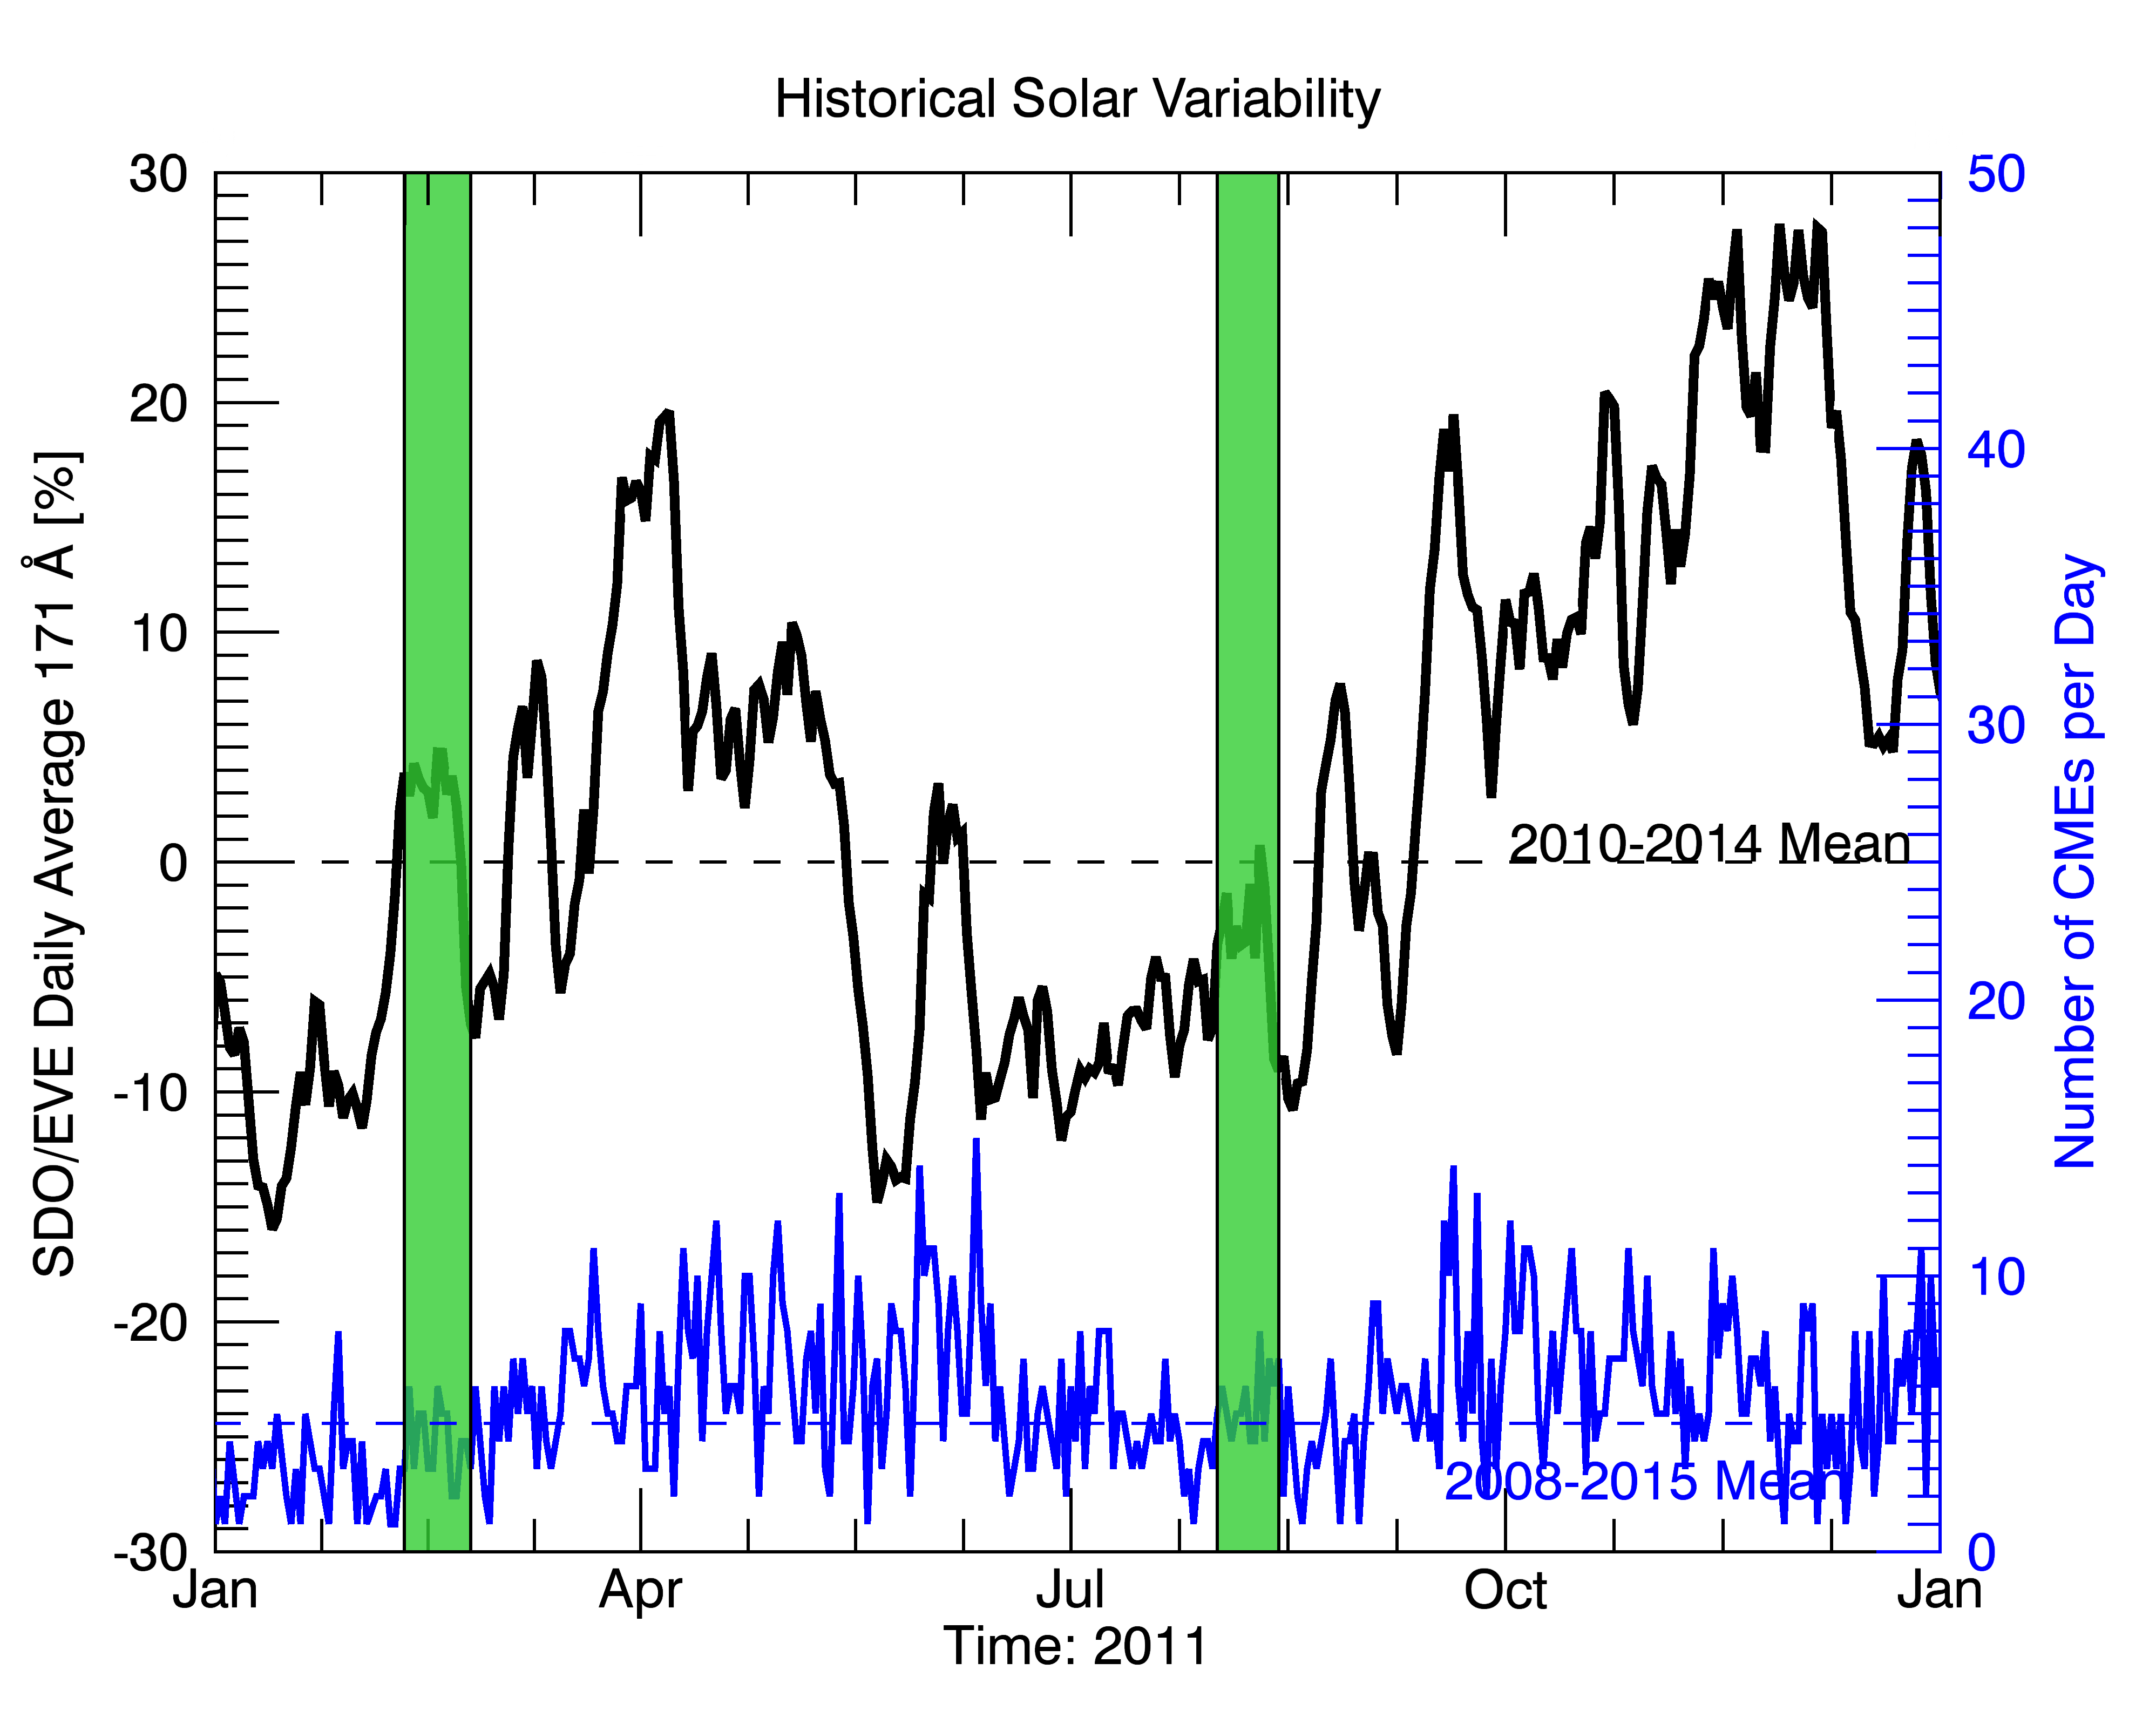
\includegraphics[width=150mm]{Images/FourWeekContext.png}
    \end{center}
    \caption[Selected four week period in historical context]{
        Context for the selected periods of study. The black line is the daily averaged EVE Fe IX 171 \AA\ line and the 
        blue line is the daily total CME occurrence. The vertical green bars indicate the selected periods of this study.
        The mean for EVE (dashed black line) is taken over the first four years of EVE's operations (2010-2014) and the 
        mean for CME occurrence (dashed blue line) is taken for the most recent solar cycle starting in 2008 to the present 
        date.
	}
    \label{fig:historicalcontext}
\end{figure}
 
Images from AIA were used to first identify dimming events. Identification was performed manually using daily AIA movies to create a list of candidate events. Two people made the identifications separately, looking at different movies. James Mason used the AIA 211-193-171 \AA\ composite movies (e.g., Figure \ref{aiacomposite2010aug7}) and Dave Webb used the 193 \AA\ movies. The primary initial selection criteria were that 1) the dimming must persist for several hours and 2) the dimming have non-trivial spatial extent e.g., at least comparable to the size of an active region. The independently identified events were then accumulated, duplicates merged as positively identified events, and disparities investigated by each identifier. Sometimes disparities proved to be questionable events according to the selection criteria above and were removed from the event list. Other times the disparities proved that the independent analysis acted as a failsafe -- a single observer simply missed an event but the other caught it. Future studies will use the automated AIA dimming detection method developed by \citet{Krista2013a}. 
 
Once the event list was deconflicted, the approximate time of the event was used to search the related observations in other instruments: flares from GOES X-ray flux, CMEs from LASCO and COR, and solar irradiance from EVE. This initial list included 38 events (includingw the 2010 August 7 simple case from Chapter \ref{chaptercasestudy}, which was outside the four week period). In some cases, the dimming was not clear in EVE data or the CME was not clearly identified in the coronagraph images; nevertheless these were dimmings identified in AIA and are listed in Table \ref{tab:eventlist} for completeness. Appendix \ref{appendixeventlist} expands the event list with ancillary data such as dimming and CME parameterization values. 29 of these events could be parameterized with EVE, 21 had measured CME velocities, and 17 had measured CME masses. Six of the CMEs had at least 2 views so that 3-D analysis could be applied for improved accuracy of the CME kinetic parameters.

\newpage
\begin{singlespace}
\begin{table}[H]
    \caption[Semi-statistical study event list]{
        Event list. Times and locations are approximate. The “derived parameters” columns abbreviations are as follows: V = 
        velocity, M = mass, 3V = 3-D velocity, 3M = 3-D mass, D = depth, S = slope. Only 29 of the events have dimming and 
        CME derived parameters to allow the study of the relationships between dimmings and CMEs. 
        See Appendix \ref{appendixeventlist} for event list with ancillary data. 
    }
    \begin{center}
    \begin{tabular}{|l|l|l|l|p{2.0cm}|p{2.0cm}|} \hline
	Event \# & Date & Time [UT] & Location & EVE \ \ \ \ \ \ \ Derived Parameters & CME Derived Parameters \\ \hline \hline
	1 & 2011 Feb 10 & 07:40 & N20 W-limb & D, S & -- \\ \hline
	2 & 2011 Feb 10 & 13:36 & N20 W-limb & D, S & V, M  \\ \hline
	3 & 2011 Feb 11 & 07:46 & N20 W-limb & D, S & V, M \\ \hline
	4 & 2011 Feb 11 & 13:21 & N60 W00 & D, S & -- \\ \hline
	5 & 2011 Feb 11 & 21:43 & N10 E-limb & D, S & V, M \\ \hline
	6 & 2011 Feb 12 & 06:05 & N30 E10 & D, S & -- \\ \hline
	7 & 2011 Feb 13 & 14:00 & S10 E10 & D, S & 3V, 3M \\ \hline
	8 & 2011 Feb 14 & 15:45 & S10 W00 & D, S & V, M \\ \hline
	9 & 2011 Feb 14 & 17:36 & N30 E20 & -- & 3V, 3M \\ \hline
	10 & 2011 Feb 15 & 02:07 & N00 W00 & D, S & 3V, 3M \\ \hline
	11 & 2011 Feb 16 & 14:40 & S20 W30 & D, S & -- \\ \hline
	12 & 2011 Feb 17 & 00:47 & E40 W00 & D, S & -- \\ \hline
	13 & 2011 Feb 18 & 11:15 & S10 W50 & D, S & V, M \\ \hline
	14 & 2011 Feb 17 & 19:20 & N30 W00 & D, S & -- \\ \hline
	15 & 2011 Feb 24 & 07:40 & N10 E-limb & D, S & -- \\ \hline
	16 & 2011 Feb 25 & 07:00 & N45 E60 & D, S & V, M \\ \hline
	17 & 2011 Aug 2 & 05:10 & N05 W20 & D, S & V, M \\ \hline
	18 & 2011 Aug 2 & 13:00 & N00 E-limb & D, S & -- \\ \hline
	19 & 2011 Aug 3 & 13:43 & N05 W48 & D, S & V, M \\ \hline
	20 & 2011 Aug 4 & 04:12 & N05 W58 & D, S & V, M \\ \hline
	21 & 2011 Aug 4 & 04:41 & N80 W00 & -- & V \\ \hline
	22 & 2011 Aug 5 & 07:25 & S30 E50 & -- & -- \\ \hline
	23 & 2011 Aug 6 & 11:50 & S14 E10 & D, S & -- \\ \hline
	24 & 2011 Aug 6 & 18:25 & N05 W25 & -- & -- \\ \hline
	25 & 2011 Aug 6 & 17:35 & N30 W-limb & -- & V, M \\ \hline
	26 & 2011 Aug 6 & 22:40 & N10 W25 & D, S & -- \\ \hline
	27 & 2011 Aug 7 & 04:00 & N10 W55 & D, S & V, M \\ \hline
	28 & 2011 Aug 8 & 01:15 & N80 E05 & -- & -- \\ \hline
	29 & 2011 Aug 8 & 11:00 & N15 W70 & -- & -- \\ \hline
	30 & 2011 Aug 8 & 17:42 & N05 W05 & D, S & -- \\ \hline
	31 & 2011 Aug 8 & 18:42 & N05 W75 & -- & 3V, 3M \\ \hline
	32 & 2011 Aug 9 & 08:10 & N15 W70 & D, S & 3V, 3M \\ \hline
	33 & 2011 Aug 9 & 09:12 & S30 E-limb & -- & -- \\ \hline
	34 & 2011 Aug 9 & 11:26 & N05 W00 & D, S & V, M \\ \hline
	35 & 2011 Aug 11 & 10:23 & N00 W-limb & D, S & 3V, 3M \\ \hline
	36 & 2011 Aug 12 & 00:09 & N45 E80 & D, S & V, M \\ \hline
	37 & 2011 Aug 12 & 11:13 & N50 E70 & D, S & -- \\ \hline
	38 & 2010 Aug 7 & 18:05 & N05 E60 & D, S & 3V, 3M \\ \hline
	\end{tabular}
    \\ \rule{0mm}{5mm}
    \end{center}
    \label{tab:eventlist}
\end{table}
\end{singlespace}

Because EVE irradiance observations are spatially integrated, dimmings from spatially-distant areas that occur too closely in time overlap in the irradiance time series and cannot be easily separated and parameterized. Thus, such events have a ``--" in Table \ref{tab:eventlist} and are excluded from the correlative study in Section \ref{sec:correlation}. This was the case for Events 9, 21, 29, 31, and 33. Similarly, Event 22 was a series of small eruptions from an active region with multiple slow CMEs whose analysis would be difficult. Secondly, some dimmings identified in AIA were not detectable in the EVE data making parameterization impossible. Here, ``not detectable" simply means that the EVE light curves did not show anything resembling the archetypal dimming near the time that was identified in AIA. This implies the magnitude of the dimming was small ($<$ 1\% impact on irradiance), which would be the case if the dimming itself was not very deep or if evolution elsewhere on the solar disk dominated (e.g., active region evolution). Examples of the former are Event 24, which was a very slight darkening of an active region’s coronal loops with no identified CME; Event 28, which was a small occurrence of ``coronal rain", also with no identified CME; and Event 25, which was an off-disk dimming event with a narrow CME. In principle, it is possible for off-disk events to generate a large irradiance change, but in this case the change was insufficient to be observable by EVE. In total, these criteria on EVE measurements resulted in 9 of the 38 events being excluded from the correlation analysis, leaving 29 events. These 29 can be processed using the flare-dimming deconvolution method described in Section \ref{sec:deconvolve}. The next section will discuss the results of this process. 

\section{Flare-Dimming Deconvolution Method Statistics}
\label{sec:deconvolutionstatistics}
There are 30 permutations of the dimming (171, 177, 180, 195, 202, 211 \AA) and nondimming (211\footnote{Again, note that 211 \AA\ is included in both dimming and nondimming categories to reflect its ambiguity}, 284, 335, 94, 131 \AA) lines for the correction method. Each one is processed using the same algorithm described in Section \ref{sec:deconvolve}. Figure \ref{fig:deconvolutioncombinations} shows an example of all 30 combinations for a single event (Event 20). It can be seen that the the higher the ionization state of the nondimming line, the "purer" the flare light curve, i.e., higher ionization states return almost perfectly back to their pre-flare irradiance level soon after the peak while lower ones show some additional response. Because the most intense heating occurs early in the flare, during the impulsive phase as observed by e.g., GOES or RHESSI HXRs, it's unlikely that the emission from high ionization states disappears because it was heated to the next ionization state. Rather, it returns to its preflare level because the intense heating supporting its existence is over and cooling has set in. Indeed, the mid-ionization states such as Fe XVI at 335 \AA\ show a slow, hours long, ramp downward in irradiance. The fact that these mid-ionization states don't immediately return back to their preflare level indicates that either the net cooling rate at those temperatures is slower than at higher temperatures and that the cooling is ongoing during this hours-long period. In other words, warm ions like Fe XVI are slowly gaining back electrons and acting as a source to the cooler ionization population like Fe IX. Critically, this ``feeding" of the Fe IX population is a cooling mechanism, not a mass-loss one. By removing this trend as indicated by the irradiance in e.g., Fe XV 284 \AA, we obtain a light curve more sensitive to mass-loss than temperature evolution (black curve in Figure \ref{fig:deconvolutioncombinations}). 

In Chapter \ref{chaptercasestudy}, it was found that for the 2010 August 7 event, the combination of Fe IX 171 Å (dimming) and Fe XV 284 Å (non-dimming) in EVE gave the best match to the spatially isolated dimming in AIA 171 \AA. The only dimming mechanisms identified to be important in this event were mass-loss and thermal. Thus, it seems that the 171 \AA\ - 284 \AA\ combination can successfully mitigate the impact of thermal processes on the dimming line. If other dimming mechanisms play an important role in the irradiance, as is the case for the 2011 August 4 case in Chapter \ref{chaptercasestudy}, it may be necessary to account for them such as by identifying and removing the impact of obscuration dimming. Until such an analysis is performed, we apply the deconvolution method to the additional 28 events with viable EVE data using the clean removal of the flare peak as the criteria for determining the best combination of dimming-nondimming line. In other words, the peaks of the dimming and scaled/time-shifted nondimming lightcurves should be similar in shape. Figure \ref{fig:deconvolutioncombinations} shows that many of combinations would meet this criteria. The next determining factor is depth of dimming. Event 20 had a relatively consistent depth of dimming for all dimming lines, but this is not the case for all events. Generally, we prefer a larger magnitude dimming as its interpretation is less ambiguous and less susceptible to being dominated by other physical processes such as active region evolution. As was shown in Chapter \ref{chaptermechansism}, the ionization level is inversely proportional to depth of dimming. Thus, 171 \AA\ is generally preferred as the dimming line but is evaluated on a case by case basis for the events studied here. Finally, all other things being equal, we prefer to use 284 \AA\ as the nondimming line for deconvolution based on the physical motivation provided in the paragraph above. 

\begin{figure}[!h]
    \begin{center}
	    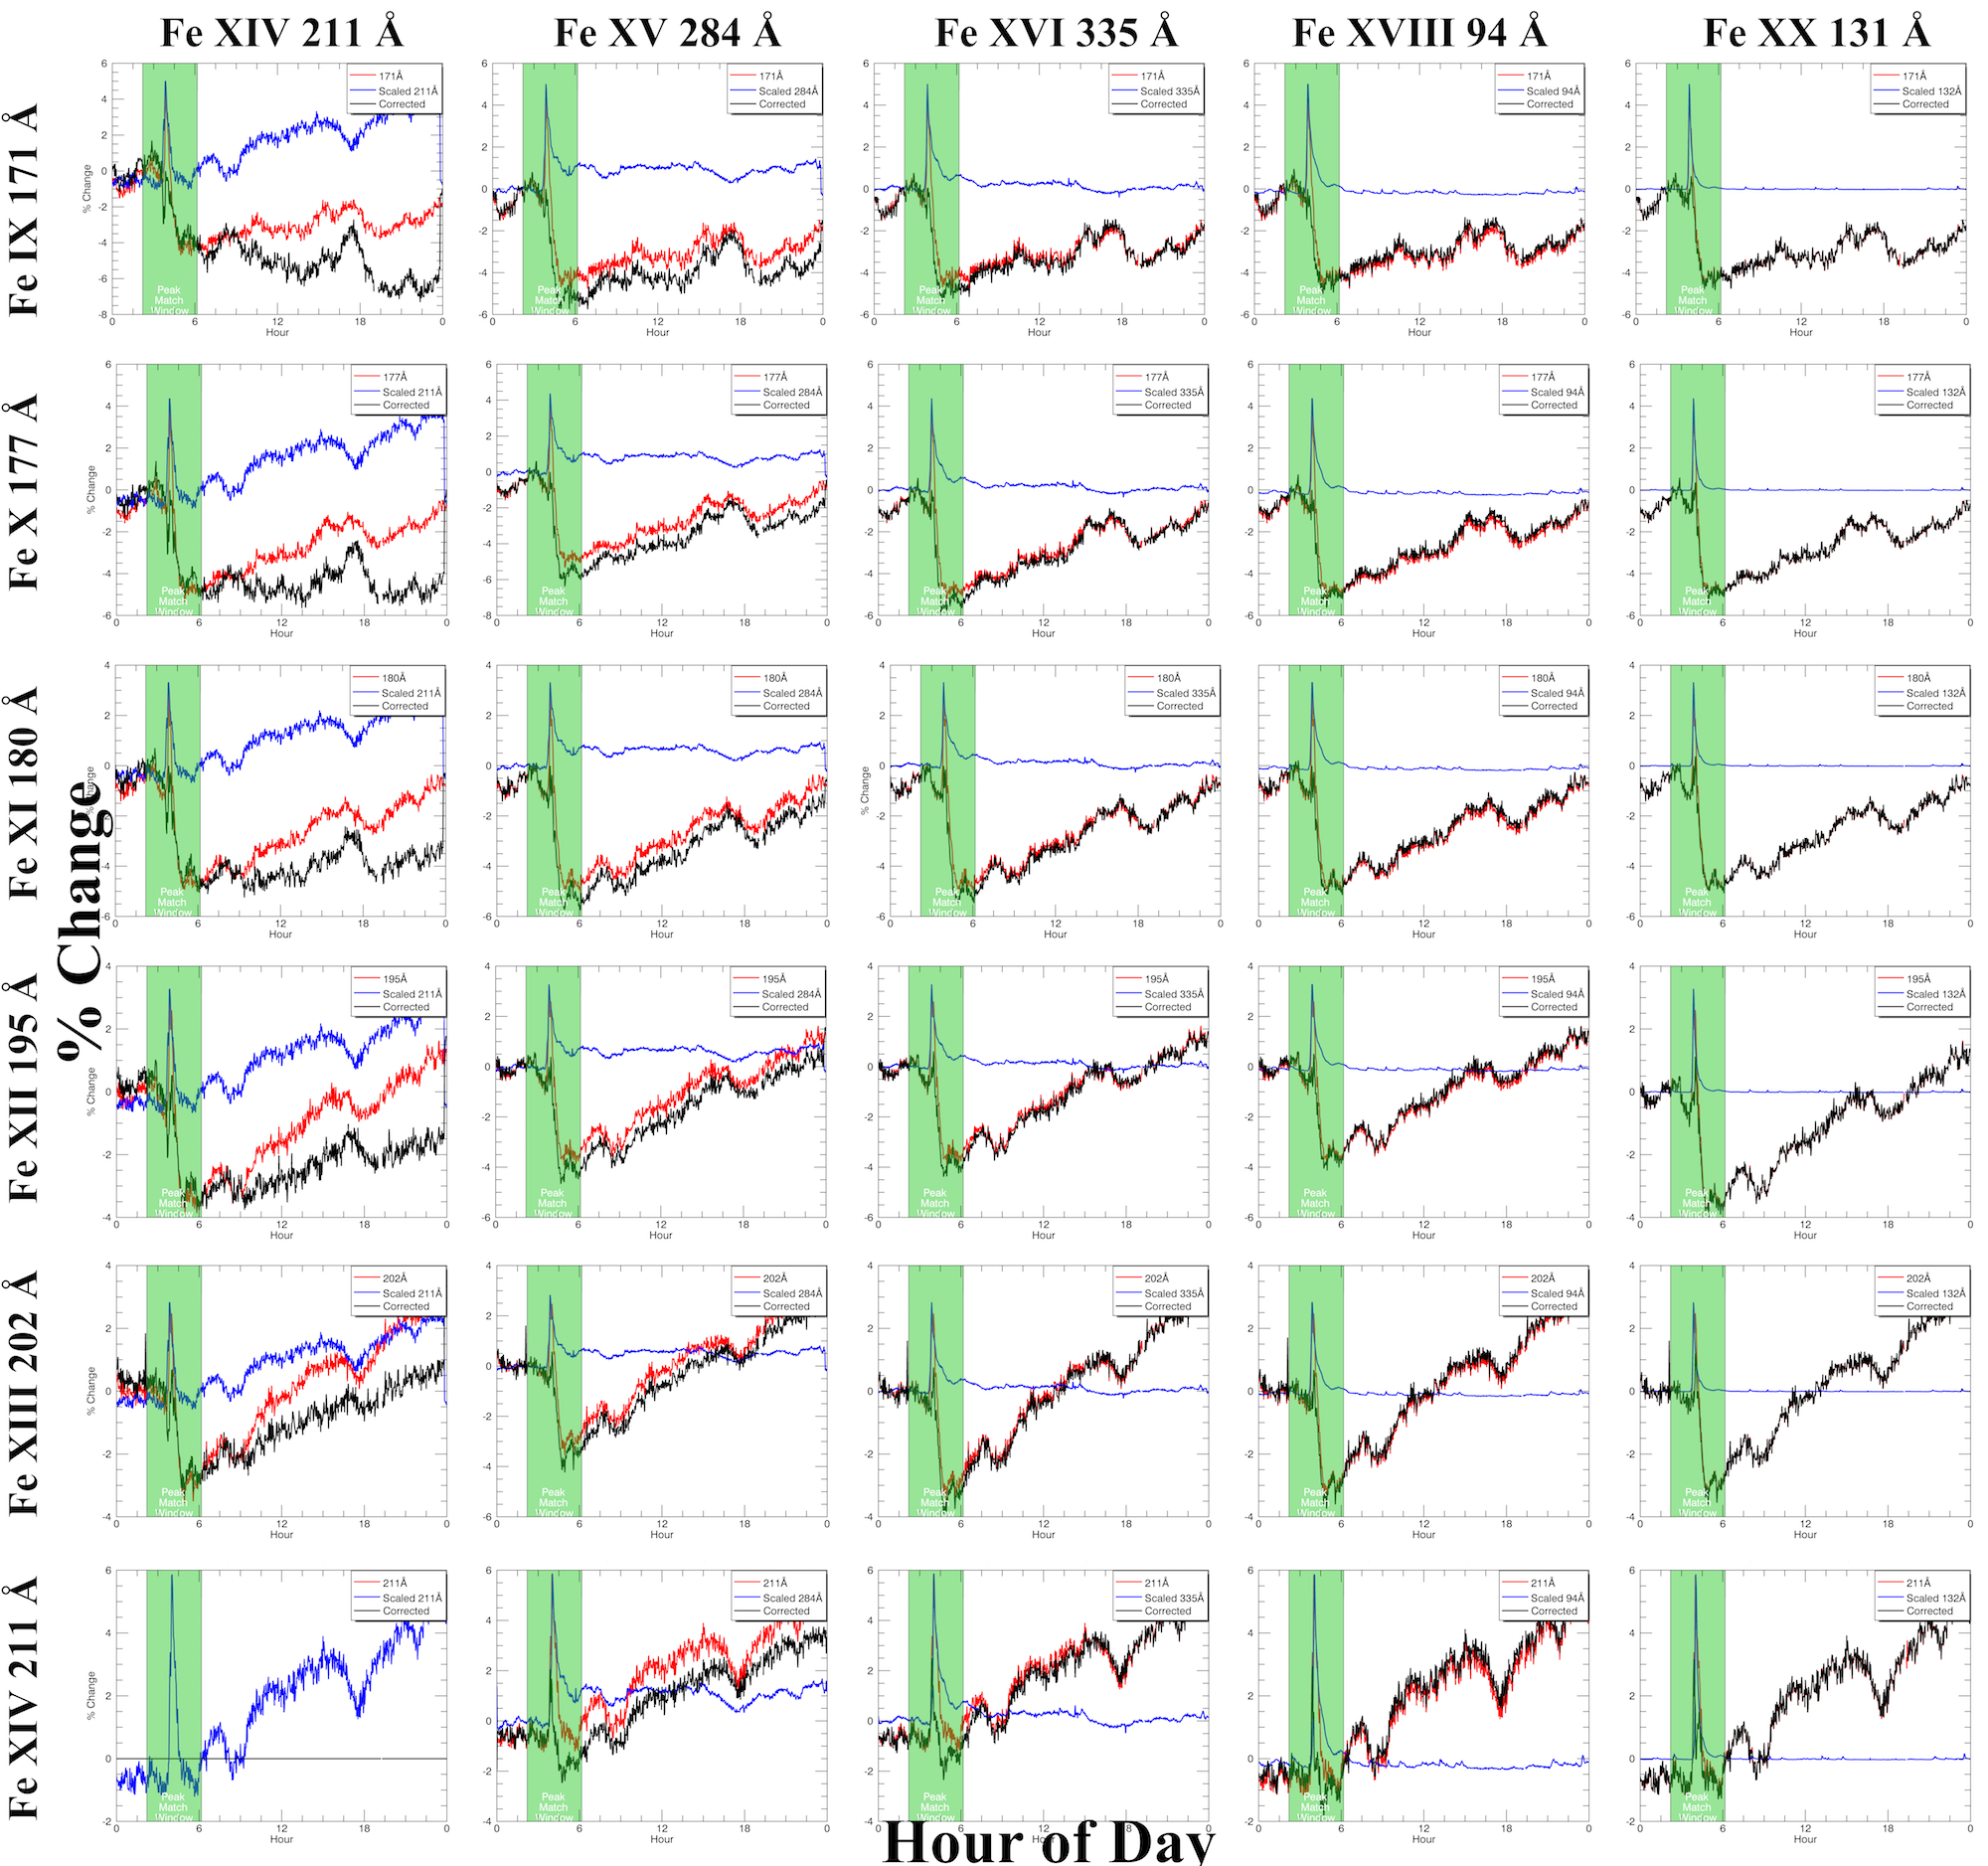
\includegraphics[width=\textwidth]{Images/AllDeconvolutionsEvent20.png}
    \end{center}
    \caption[All deconvolution combinations example]{
        Example of every combination of the dimming (rows) and nondimming (columns) lines for the deconvolution method for 
        a single event (Event 20). In each plot, the red is the dimming line, blue is the scaled and time shifted 
        nondimming line, and black is the result of the subtraction (red - blue). The vertical transparent green bar 
        indicates the time window the algorithm uses for finding and matching peaks. 
   	}
    \label{fig:deconvolutioncombinations}
\end{figure}

This methodology has been applied to the 28 unique EVE dimmings found during the four weeks studied. Of these, all 28 were found to be best represented by the 171 \AA\ - 284 \AA\ combination. It is possible that other coronal line pairings might be better for different spectral resolution measurements. We will gain additional confidence in the effectiveness of this line pairing for EVE if we find a positive and statistically significant correlation between corrected EVE light curve parameterizations to independently derived CME mass and velocity. The first step in that process is to fit the EVE light curves in preparation for dimming parameterization. 

\section{Dimming Light Curve Fitting Method}
\label{sec:fittingmethod}

\subsection{Physics Motivation and Fit Types}
The $\beta$ parameter for a plasma is an indicator of the relative importance of plasma and magnetic pressures, expressed as 

\begin{equation*}
    \beta = \frac{p_{plasma}}{p_{mag}} = \frac{nk_bT}{B^2/(2\mu _0)}
\end{equation*}

\noindent where $p$ is pressure, $n$ is number density, $k_b$ is Boltzmann's constant, $T$ is temperature, $B$ is magnetic field strength, and $\mu _0$ is the permeability of free space. In the solar corona, $\beta$ is typically < 1, indicating that the magnetic field dominates the flow of plasma, i.e. plasma is confined by magnetic fields. Thus, in the initiation of a CME where magnetic fields are propelled out of the corona and expand as they do so, the plasma in the enclosed bubble of the CME experiences an adiabatic expansion and density decrease (Figure \ref{fig:limbcmedimming}). \citet{Aschwanden2009a} described this process and here we adapt it for the variation of intensity in collisionally-excited lines as a function of height for a constant-temperature and expanding volume:

\begin{equation}
    \frac{I(t)}{I_0} \propto \left(\frac{h_0}{h(t)}\right)^3
    \label{eq:irradiancevsheight}
\end{equation}

where $I(t)$ is the bubble intensity as a function of time $t$, $I_0$ is the intensity at an initial time, and $h$ is the corresponding height. Note that height as a function of time is a speed. This simple power-law description does not account for any complicating factors such as thermally-induced emission changes, interaction with overlying coronal magnetic fields, or later recovery of the regional emission. \citet{Aschwanden2009b} developed a more sophisticated model of dimmings, including adiabatic expansion and gravitational stratification. However, the model contains 14 free parameters and is more suited to a case-by-case study of dimming morphologies. For the purposes of our correlative study, it is reasonable to assume that the decrease in emission due to the volume density is more significant than the thermal and inhomogeneity effects, and that the effective height scale of the CME is the most important parameter. 

\begin{figure}[!h]
    \begin{center}
	    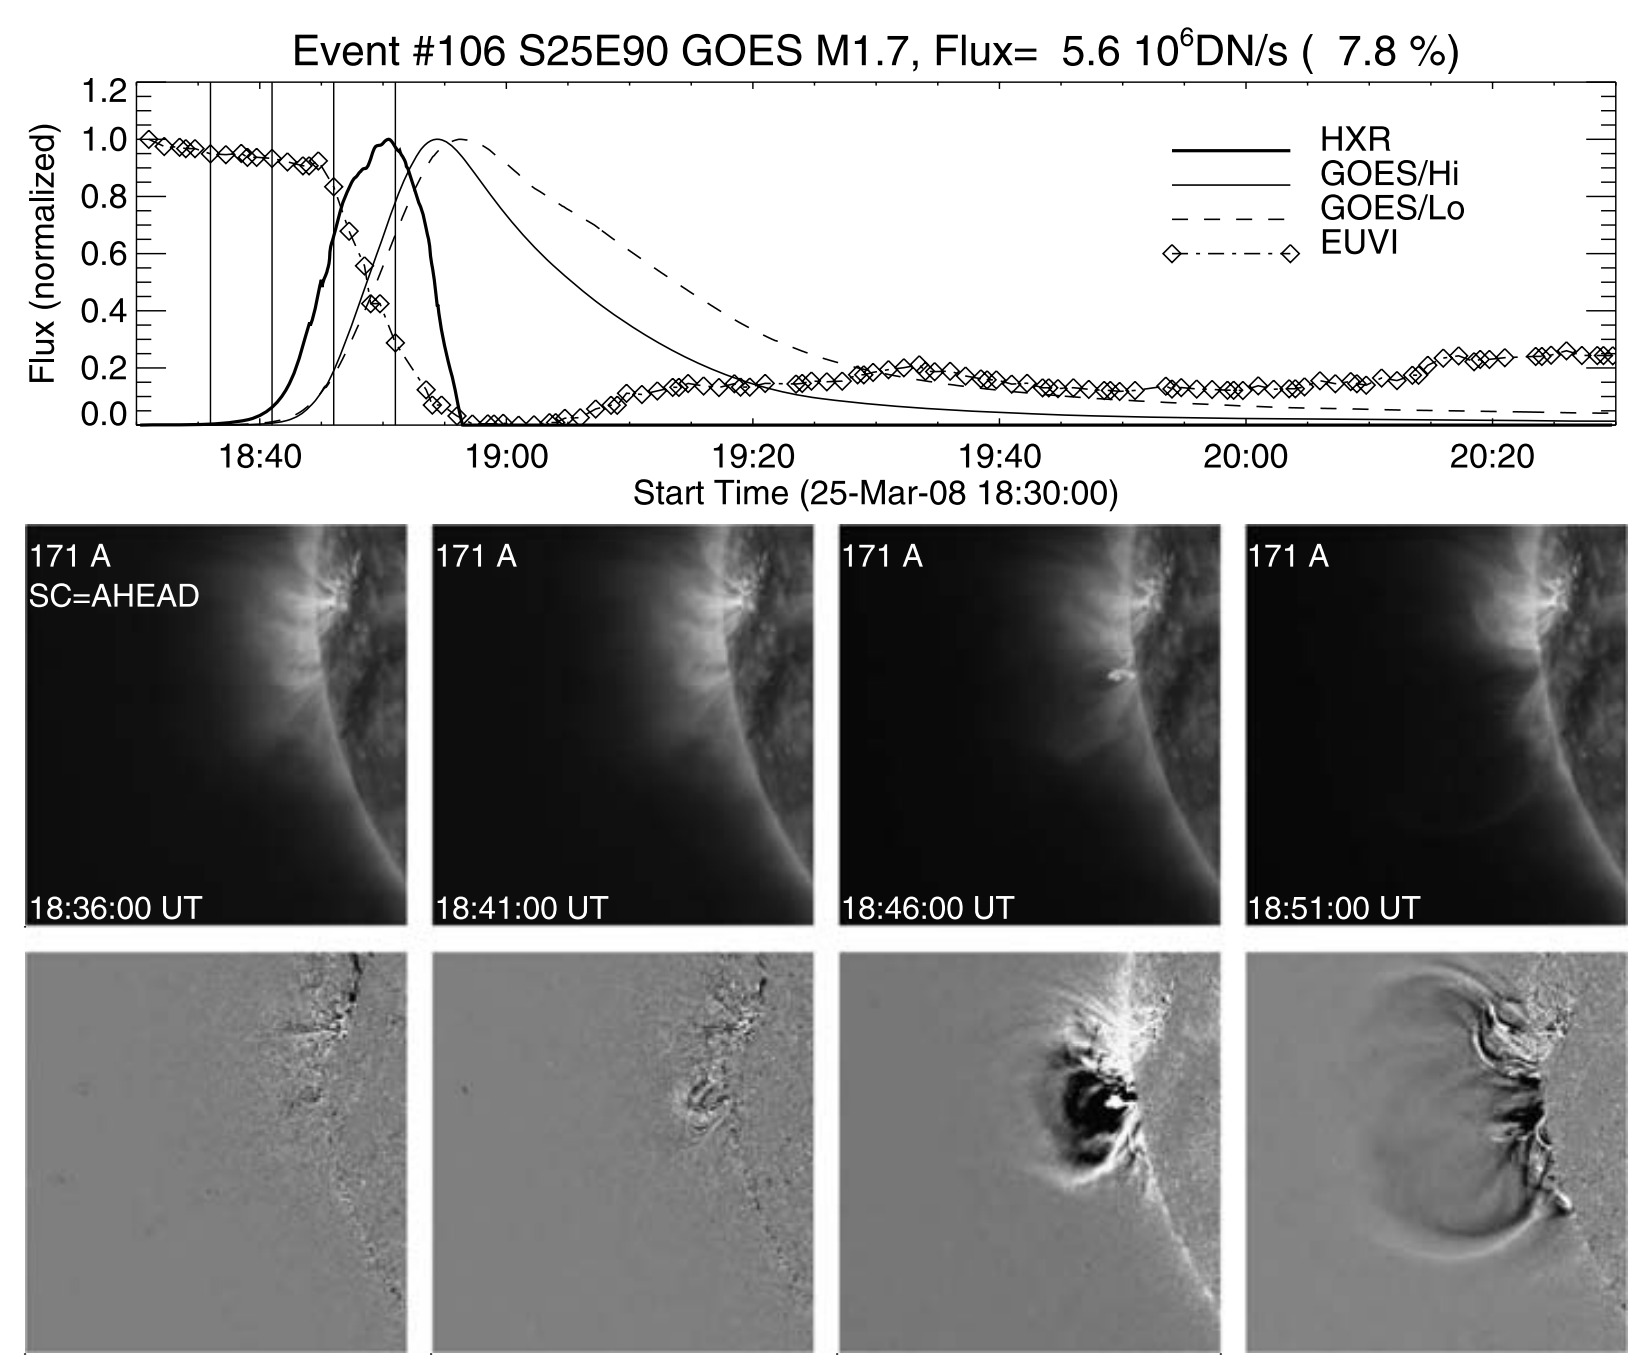
\includegraphics[width=\textwidth]{Images/CMEExpansionLimb.png}
    \end{center}
    \caption[Limb CME expansion and dimming]{
        Example of CME bubble expansion and associated EUV dimming. (Top) Soft X-ray (GOES/Lo 0.5 – 4 Å and 1 – 8 Å, thin 
        curves) and EUV (STEREO-A/EUVI, diamonds) light curves and time derivative, dI(t)/dt, of the harder soft X-ray 
        light curve (thick solid line) for the flare/CME event on 2008 March 25 at 18:30 UT. (Bottom) Four STEREO-A/EUVI 
        images (top row) and running-difference images (bottom row). Note the strong dimming in the EUV light curve.
        The diamond symbols mark the times of the EUV images; the selected images shown below are marked with
        vertical lines. The peak EUV flux is $F = 5.6 \times 10^6 DN s^{−1}$ (or 7.8\% of the total flux). The field of 
        view of the images is 512 EUVI pixels (≈600 Mm). Adapted from \citet{Aschwanden2009a}. 
   	}
    \label{fig:limbcmedimming}
\end{figure}

In Equation \ref{eq:irradiancevsheight}, as time tends to infinity, the local emission goes to zero. However, the solar irradiance, as observed by EVE, decreases to a constant background value during a dimming event. Thus, this simple power-law fit for the EVE dimming events can not be used directly. Furthermore, the relationship of height and time is not well established, so different functions are fitted to the EVE dimming events to explore which functions are more optimal for determining the dimming event parameters of depth and slope.

Exponential and power law fits tend to result in $\chi^2 > 20$, meaning they were very poor fits. Polynomial fits up to order five were also computed, with 5th and 3rd orders appearing to best describe the shape of the light curves (see Figures \ref{fig:bestfithistogram} and \ref{fig:fitsexample}). Although the 3rd order polynomial function is expected to be a better match to the theory, the best-fit function is used for deriving the dimming slope and depth. 

\begin{figure}[!h]
    \begin{center}
	    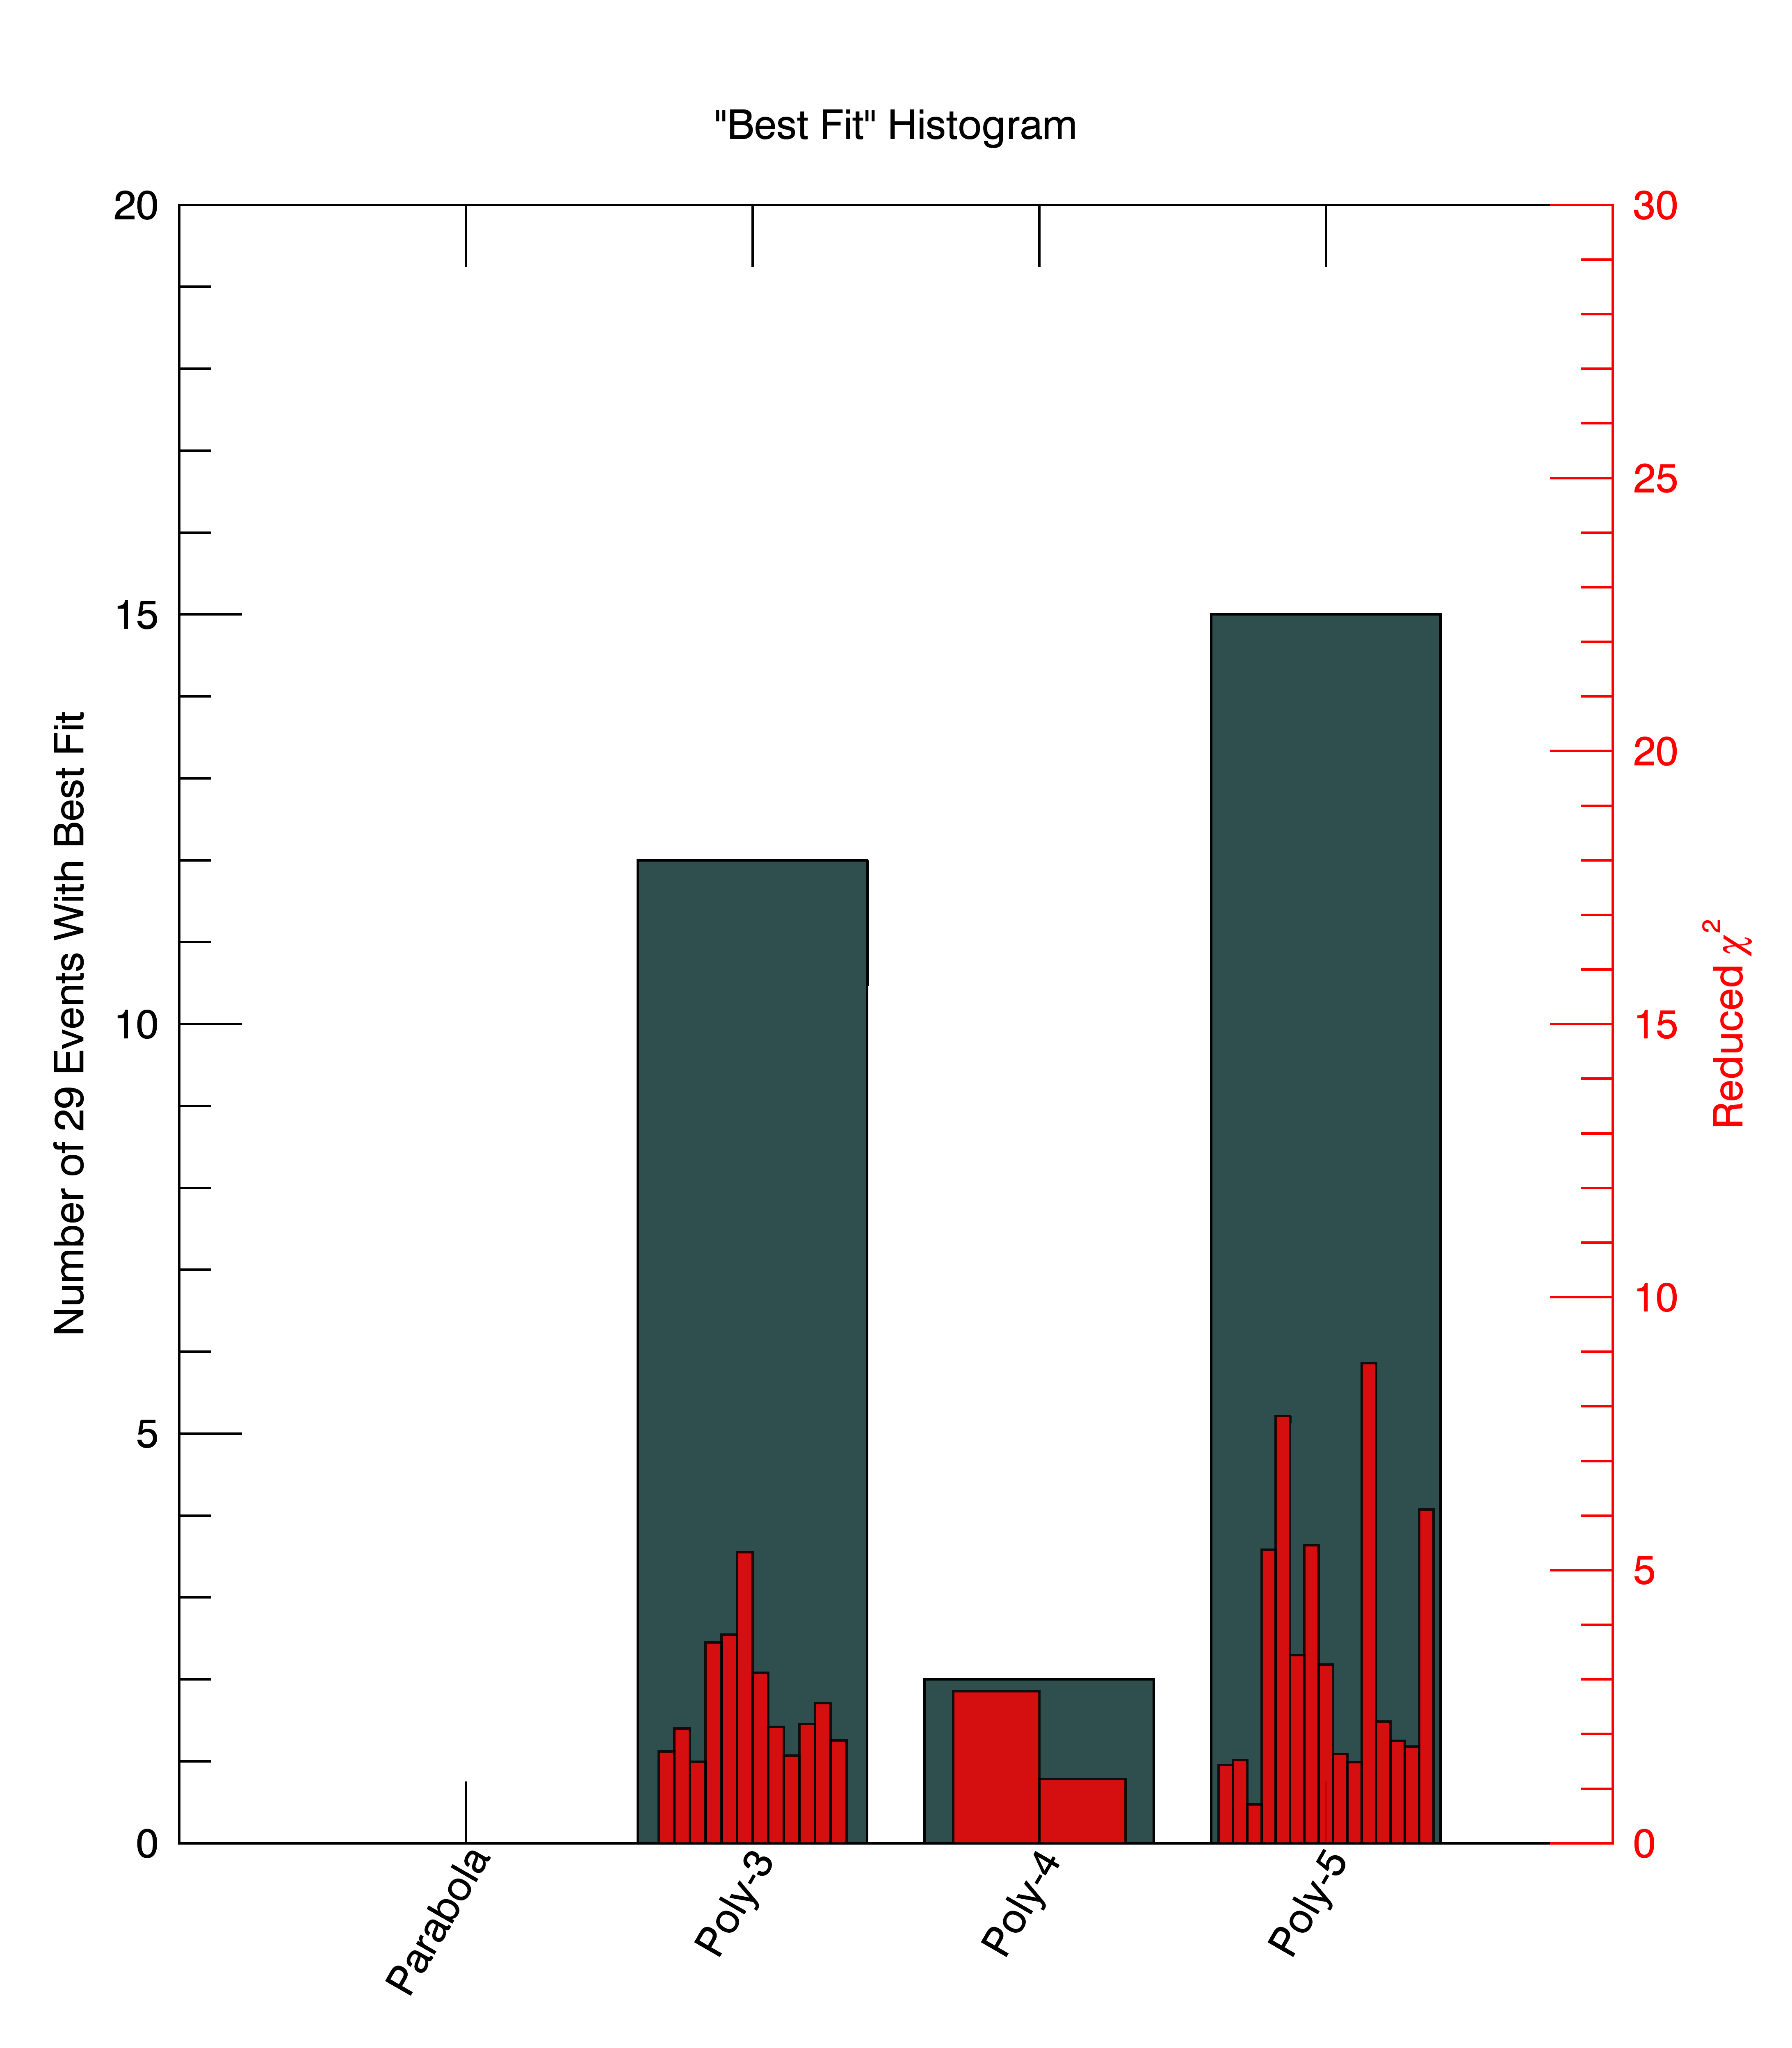
\includegraphics[width=100mm]{Images/BestFitHistogram.png}
    \end{center}
    \caption[Dimming best fit statistics]{
        (blue) Statistics of manually selected ``best fit” for all unique EVE dimming events in 4 weeks studied and 
        (red) the reduced $\chi^2$ for the best fits. The 3rd and 5th order polynomial fits provided the largest number
        of best fits.
    }
    \label{fig:bestfithistogram}
\end{figure}

\subsection{Dimming Fit Uncertainty Computation}
The uncertainties from Section \ref{sec:deconvolveerrors} correspond to the deconvolved/corrected EVE dimming light curve. Those light curves are the input for the fitting function, IDL's \textit{poly{\_}fit}, which also accepts an input \textit{measure{\_}errors} for uncertainties. Figure \ref{fig:fitsexample} shows polynomial fits from 2 to 5 with the measurement errors and the resultant $1\sigma$ uncertainties computed by \textit{poly{\_}fit}. The fits achieve the desired effect of reducing uncertainty even further and providing a smooth function to parameterize.

\begin{figure}[!h]
    \begin{center}
	    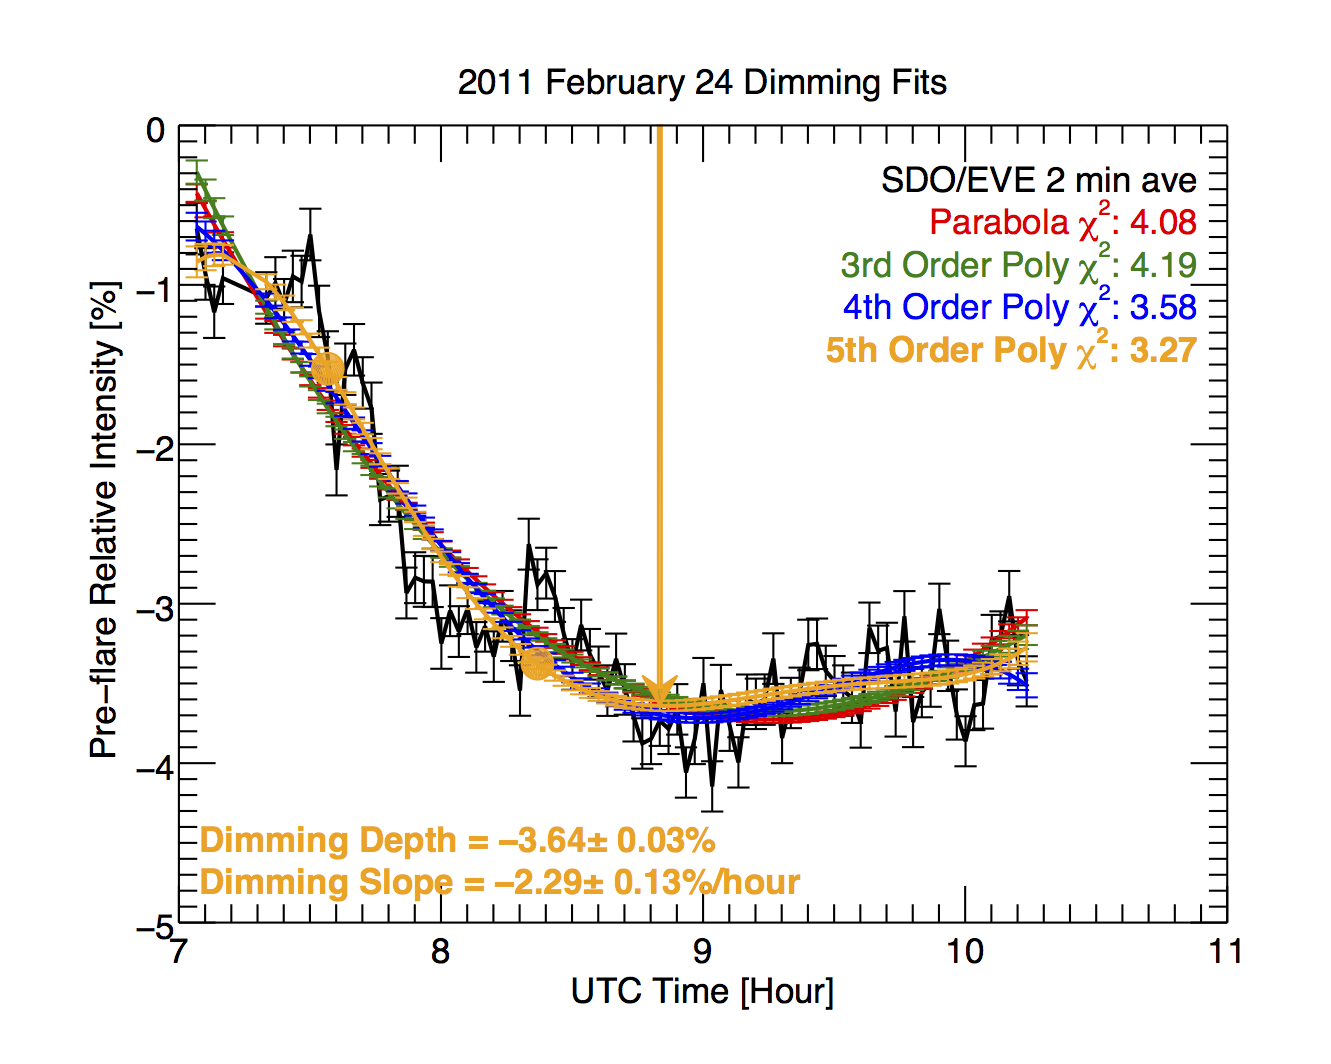
\includegraphics[width=100mm]{Images/DimmingFitsExample.png}
    \end{center}
    \caption[Dimming fits example]{
        A single dimming event (Event 15) showing the reduction in uncertainties of the fits compared to the EVE data. The
        arrow shows the location of dimming “depth” parameterization for this event, and the two filled circles indicate the 
        range where “slope” was computed. Their colors correspond to the fit types in the legend. The lowest  indicates 
        that the 5th order polynomial was the best fit for this event, but we note that the results from the other 
        polynomial fits are very similar.
   	}
    \label{fig:fitsexample}
\end{figure}

\section{Parameterization Methods}
\label{sec:parameterization}
Dimming and CMEs are complex phenomena with complex observations and associated data analysis. Our end goal is to provide simple measures of dimming to act as proxies for CME mass and speed, driven by a physical explanation. Given this, the space weather community would have an independent indicator of CME presence and importance to geospace, and the astronomy community would have a means of detecting and characterizing CMEs on other stars (albeit a first-order characterization). To that end, this section describes the parameter derivations for dimming and CMEs that will be used to establish a correlation in Section \ref{sec:correlation}, motivated by the physics in preceding sections. 

\subsection{Dimming Parameterization}
Points for the computation of slope and depth are selected manually from the best fit light curve from Section \ref{sec:fittingmethod}. Slope point selection was guided by the desire to have $\chi^2$ near unity and by some flexibility for events where the EVE dimming correction method did not completely remove the flare peak of the cool corona line (Fe IX 171 \AA). In such cases with a residual flare peak, the fits can deviate from the ``pure" dimming light curve and skew the   upward. Rather than develop a complicated algorithm to account for this effect autonomously, selection of the best fit was done by manual inspection. Dimming slope was computed across a range: the initial point was typically chosen to be soon after the initial dimming rollover when the slope becomes relatively constant, and the final point was selected just prior to the inverse rollover leading to the relatively flat period in the light curve (see solid circles Figure \ref{fig:fitsexample}). The slope need not be constant between these two points. For each time step within the selected range, the derivative was computed. The single-value slope parameter for each event is the mean of these derivative (slope) values. The dimming depth parameter is taken from a relatively stable pre-flare value to a point near the beginning of the dimming floor (see arrow in Figure \ref{fig:fitsexample}). 

The uncertainty associated with dimming depth is just the uncertainty of the fitted light curve at the point selected for the depth measure, as exemplified by the error bar at the arrow in Figure \ref{fig:fitsexample}. The uncertainty for slope requires some additional computation. To compute the derivative of the light curve at each point within the specified time range, IDL's \textit{deriv} function is used; the corresponding \textit{derivsig} function returns the $1\sigma$ uncertainty for each point in the derivative array. Collapsing the various derivatives into a single slope parameter via the mean has the corresponding uncertainty, 

\begin{equation*}
    \sigma _{slope} = \frac{1}{N}\sqrt{\sigma^2_1 + \sigma^2_2 + ... \sigma^2_n}
\end{equation*}

\noindent where N is the number of points, and $\sigma_1$...$\sigma_n$ are the uncertainties for each point returned from \textit{derivsig}. Appendix \ref{appendixeventlist} includes the dimming depth, slope, depth uncertainty, and slope uncertainty for each of the 38 events studied. 

\subsection{CME Parameterization}
The detailed 3-D analysis of the velocity and mass was possible for six of the best-observed CMEs, using either or both LASCO and the CORs data. These six events are noted as “3V, 3M” in Table \ref{tab:eventlist} and shown as solid red symbols in Figure \ref{fig:correlations}. Following the method of \citet{Colaninno2009}, the GCS model is fit to the observations to determine the 3-D location and heights of the CMEs. The 3-D heights and longitude of the CME are needed to calculate the ``true" 3-D mass of the CME. These heights are also used to calculate the de-projected velocity of the CME. The reported masses are for a height of 15 R\astrosun, using the fitting method of \citet{Bein2013} for mass increase with height. For the 2011 February 13-15 CMEs the mass was measured in both COR2A and COR2B and then averaged. For the 2011 August 9 and 11 CMEs, the mass was measured in LASCO-C3 only.

The following procedure was used to estimate the uncertainties for the CME kinetic parameters. The LASCO CDAW measurements were used for most of the events to derive the CME velocity and mass, which are based on a single viewpoint observation as opposed to 3-D. The reported linear speed of each CME is obtained by fitting a straight line fit to the height-time measurements at a fixed position angle. If we assume conservatively that the CME axis is 60\degree from the sky plane as the worst case (for non-halo CMEs), this results in a factor of 2 (50\%) underestimation of the speed. The CDAW catalog also provides the CME span angle, which can be used to provide an estimated error on the CME mass (Figure 4 of \citealt{Vourlidas2010}). As an example, if we take Event 2 from Table \ref{tab:eventlist} above, then using these errors we have $speed = 338 \pm 345 km\ s^{-1}$ and $mass = 3.40 \times 10^{14} \pm 4.30 \times 10^{14}\ g$. 

For the six events with 3-D analysis of the CME measurements, we derive the error in the speed from the linear fit to the data assuming the error in the 3-D height measurements is $\pm 0.48 R\astrosun$ \citep{Colaninno2013}. Thus, if we take Event 7 as a typical 3-D CME measurement, we get $353 \pm 13\ km\ s^{-1}$ for the speed. The mass is still considered an underestimate from the 3-D analysis but is better determined because the plane-of-sky angle and 3-D heights are known from the GCS model fit, so a $\pm 15\%$ error is assumed for the 3-D mass estimates \citep{Bein2013}.

For the purpose of linear-fitting with dimming parameters in Section \ref{sec:correlation}, the midpoint between the low and high limits is chosen for each CME speed and mass parameter reported here, and the CME parameter error is the range between the high and low limits divided by two (i.e., $\pm$ error bars in Figure \ref{fig:correlations}). The plot of the points themselves does not display this center-point for single-viewpoint derived CME parameters but does for 3-D derived CME parameters. Appendix \ref{appendixeventlist} includes the CME speed, mass, speed uncertainty, and mass uncertainty for each of the 38 events studied.

\section{Dimming and CME Parameters Correlation}
\label{sec:correlation}
As described in Chapter \ref{chaptercasestudy}, we expect direct proportionality between dimming depth and CME mass, and between dimming slope and CME velocity. In other words, there should be a stronger correlation between these parameters than between any other combination of parameters. The analysis of just two events in that chapter does not establish any such possible relationships. This study is a more in-depth examination of such possible relationships with many more events. While our intention for this study was to have ~30 events, it was challenging to obtain CME velocity and mass for all of the candidate events. Nevertheless, there was a sufficient number events with dimming and CME parameterizations to establish a significant correlation. Table \ref{tab:correlations} provides the Pearson correlation coefficients \citep{Pearson1895} and p-value permutation statistical tests between each combination of the dimming and CME parameters, which confirms our initial expectation. Smaller p-values indicate a lower probability that the correlation could have arisen if no correlation existed at all. There is positive correlation between all of the parameter permutations, which is likely due to the ``big flare syndrome" \citep{Kahler1982, Kahler1992}, e.g., a rapid, powerful coronal magnetic field energy release tends to result in a faster, more massive CME. 

\begin{table}[!h]
    \caption[Dimming-CME parameter correlations]{
        Pearson correlation coefficients (PCC) and p-values between dimming and CME parameters.
    }
    \begin{center}
    \begin{tabular}{|l|l|l|l|} \hline
	Parameter 1 & Parameter 2 & PCC & p-value \\ \hline \hline
	Slope & Speed & 0.78 & $1.51 \times 10^{-4}$ \\ \hline
	Depth & Mass & 0.74 & $7.80 \times 10^{-4}$ \\ \hline
	Slope & Mass & 0.60 & 0.01 \\ \hline
	Depth & Speed & 0.51 & 0.04 \\ \hline
	Mass & Speed & 0.64 & $2.79 \times 10^{-3}$ \\ \hline
	Slope & Depth & 0.27 & 0.15 \\ \hline
	\end{tabular}
    \\ \rule{0mm}{5mm}
    \end{center}
    \label{tab:correlations}
\end{table}

\begin{figure}[!h]
    \begin{center}
	    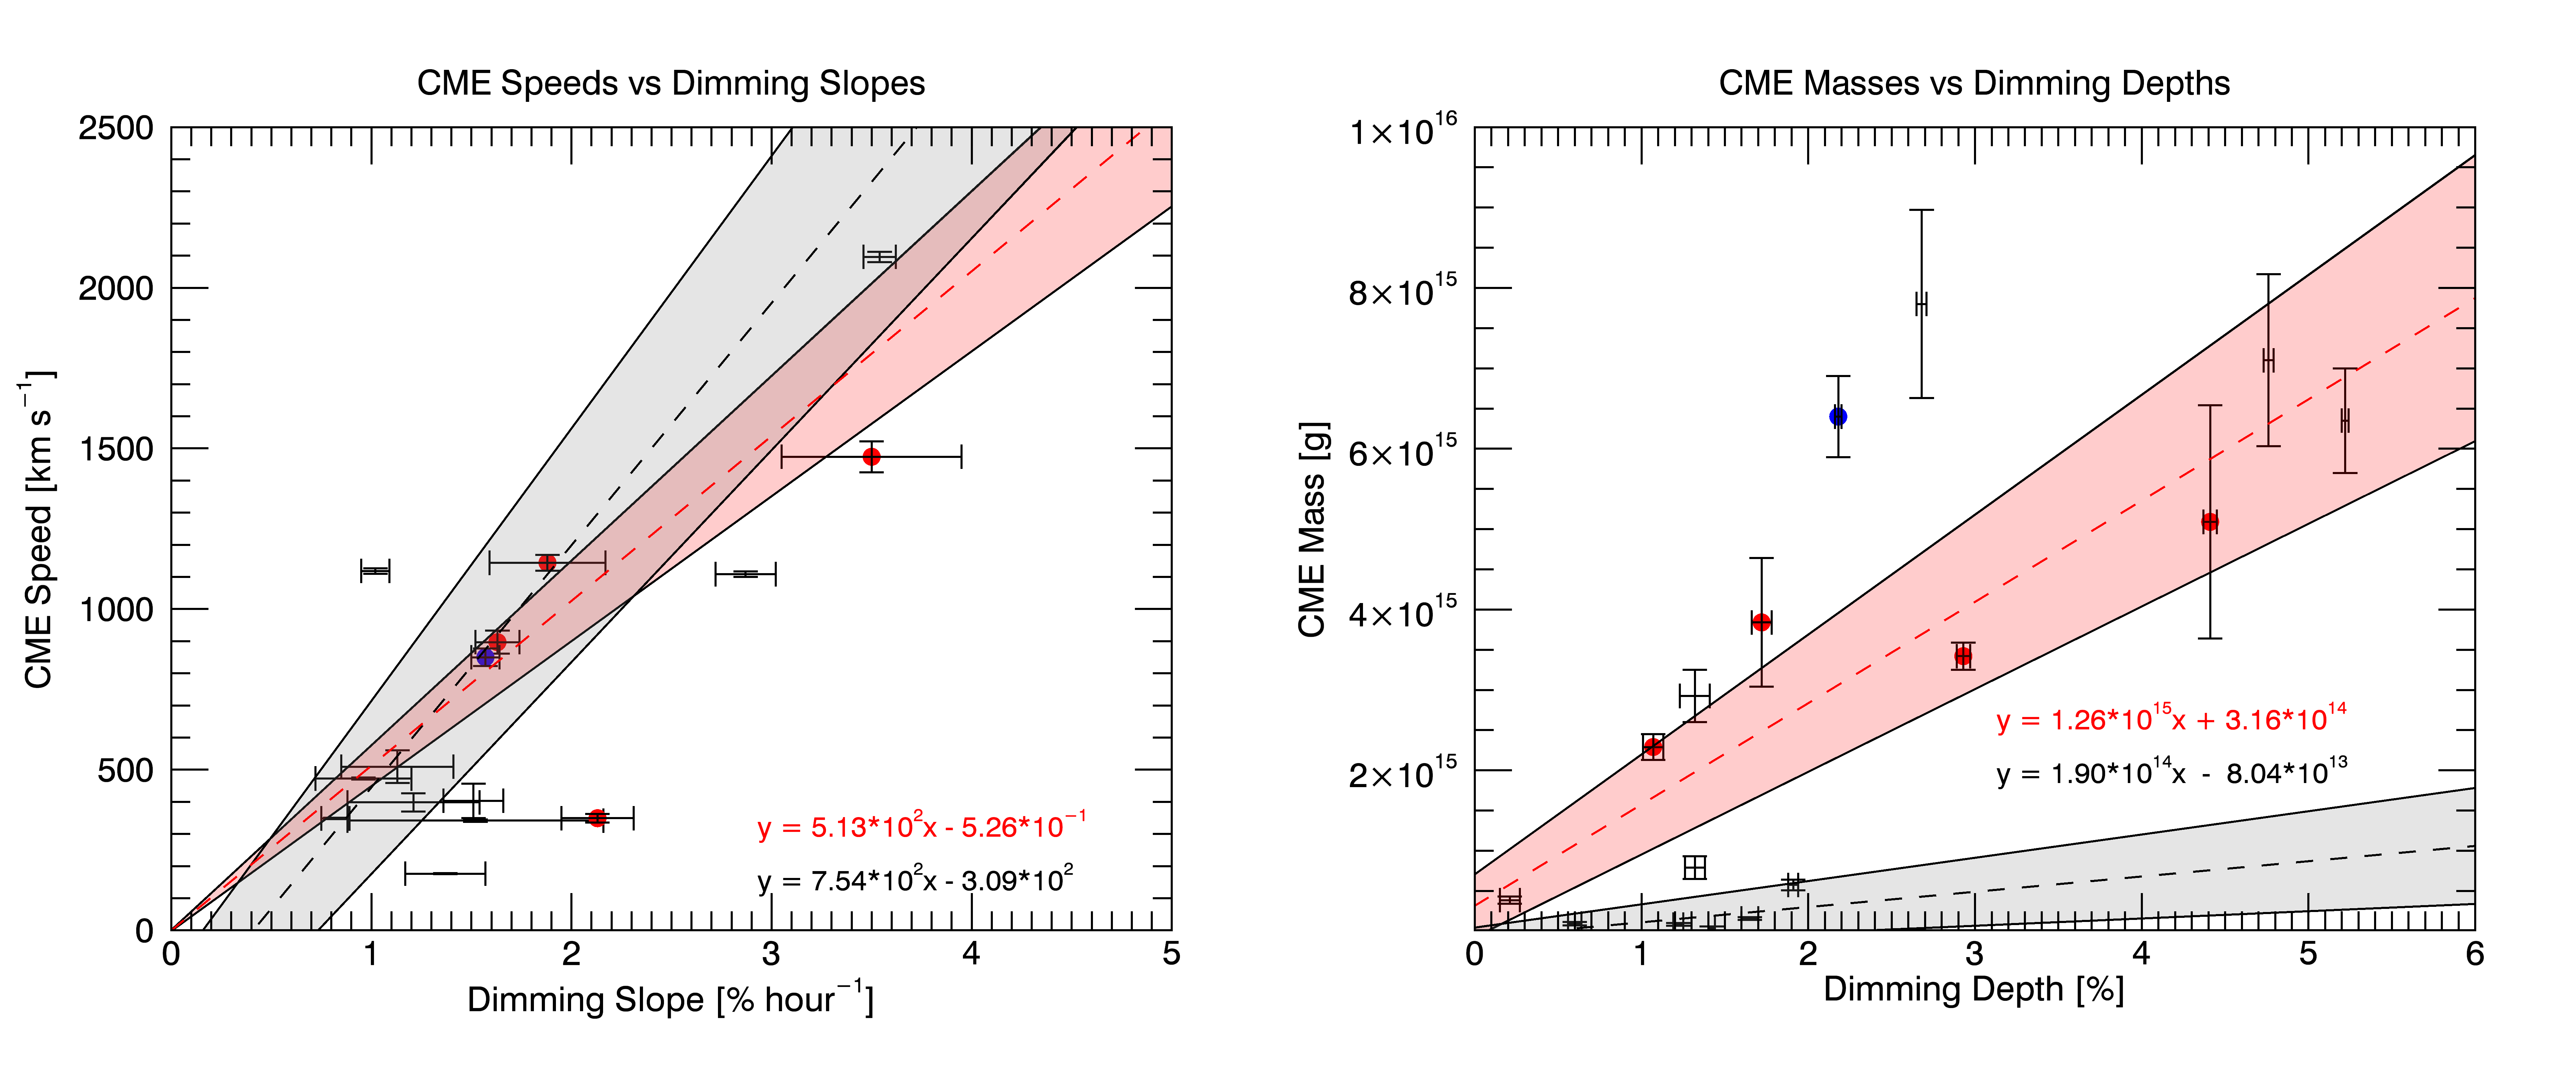
\includegraphics[width=\textwidth]{Images/Correlations.png}
    \end{center}
    \caption[Dimming-CME correlations]{
        Scatterplots of (left) CME speed and dimming slope and (right) CME mass and dimming depth. Data without a 
        center-point are derived from a single viewpoint of CMEs and are thus presented as a range of possible values 
        rather than a single point with a standard uncertainty. Red symbols, line, and text indicate 3-D computed CME 
        parameters, and the blue symbol indicates data from the simple 2010 August 7 event, which is also 3-D derived. 
        Linear fits are shown as the dashed lines, and the grey/pink region represents the 3σ uncertainty of the linear 
        fits.
   	}
    \label{fig:correlations}
\end{figure}

Figure \ref{fig:correlations} shows scatterplots of speed vs. slope and mass vs. depth with estimated error bars. Linear fits for each scatterplot were computed using IDL's \textit{fitexy}, which can accept input errors in both axes and return the fit parameters with a $1\sigma$ uncertainty. The fit uncertainty is converted to $3\sigma$ and used to define the grey/pink regions of Figure \ref{fig:correlations}. The fit equations are also listed in the Figure \ref{fig:correlations} panels. This process was repeated using only CME values computed from the 3-D methods and are plotted as the red dashed line and pink shaded region. In order to get a nominal fit for the 3-D case with so few data points, a virtual (0, 0) point was added to the fit. 

The mass vs. depth plot (Figure \ref{fig:correlations}, right) is linear-linear for clarity of the fits, but several of the data points end up off scale as they are $< 1 \times 10^{15}\ g$. These points skew the fit uncertainty (grey area) significantly. Figure \ref{fig:correlationshighlowmass} is analogous to Figure \ref{fig:correlations}, but shows the fit applied to high-mass only and low-mass only separately. The fit for high-mass only shows a slope that is less than a factor of two different from the all-points and 3-D points fits, whereas the fit for low-mass shows a slope that is an order of magnitude different from the others. When ignoring the low-mass points, the fit uncertainty narrows and is less skewed (grey area) and nearly all points fall within the uncertainty, when accounting for the uncertainty of the individual mass points. Thus, we suspect there may be two statistical families in the data. We examined all of these events individually and didn’t notice any dimming or CME peculiarities that might cause this separation of high-mass and low-mass families in this comparison. The families do not strongly correlate to GOES flare magnitude (or whether there was a flare at all), CME span, or flare type. This result may be an artifact of small number statistics, which could be remedied in future work with many more dimming-CME events. 

\begin{figure}[!h]
    \begin{center}
	    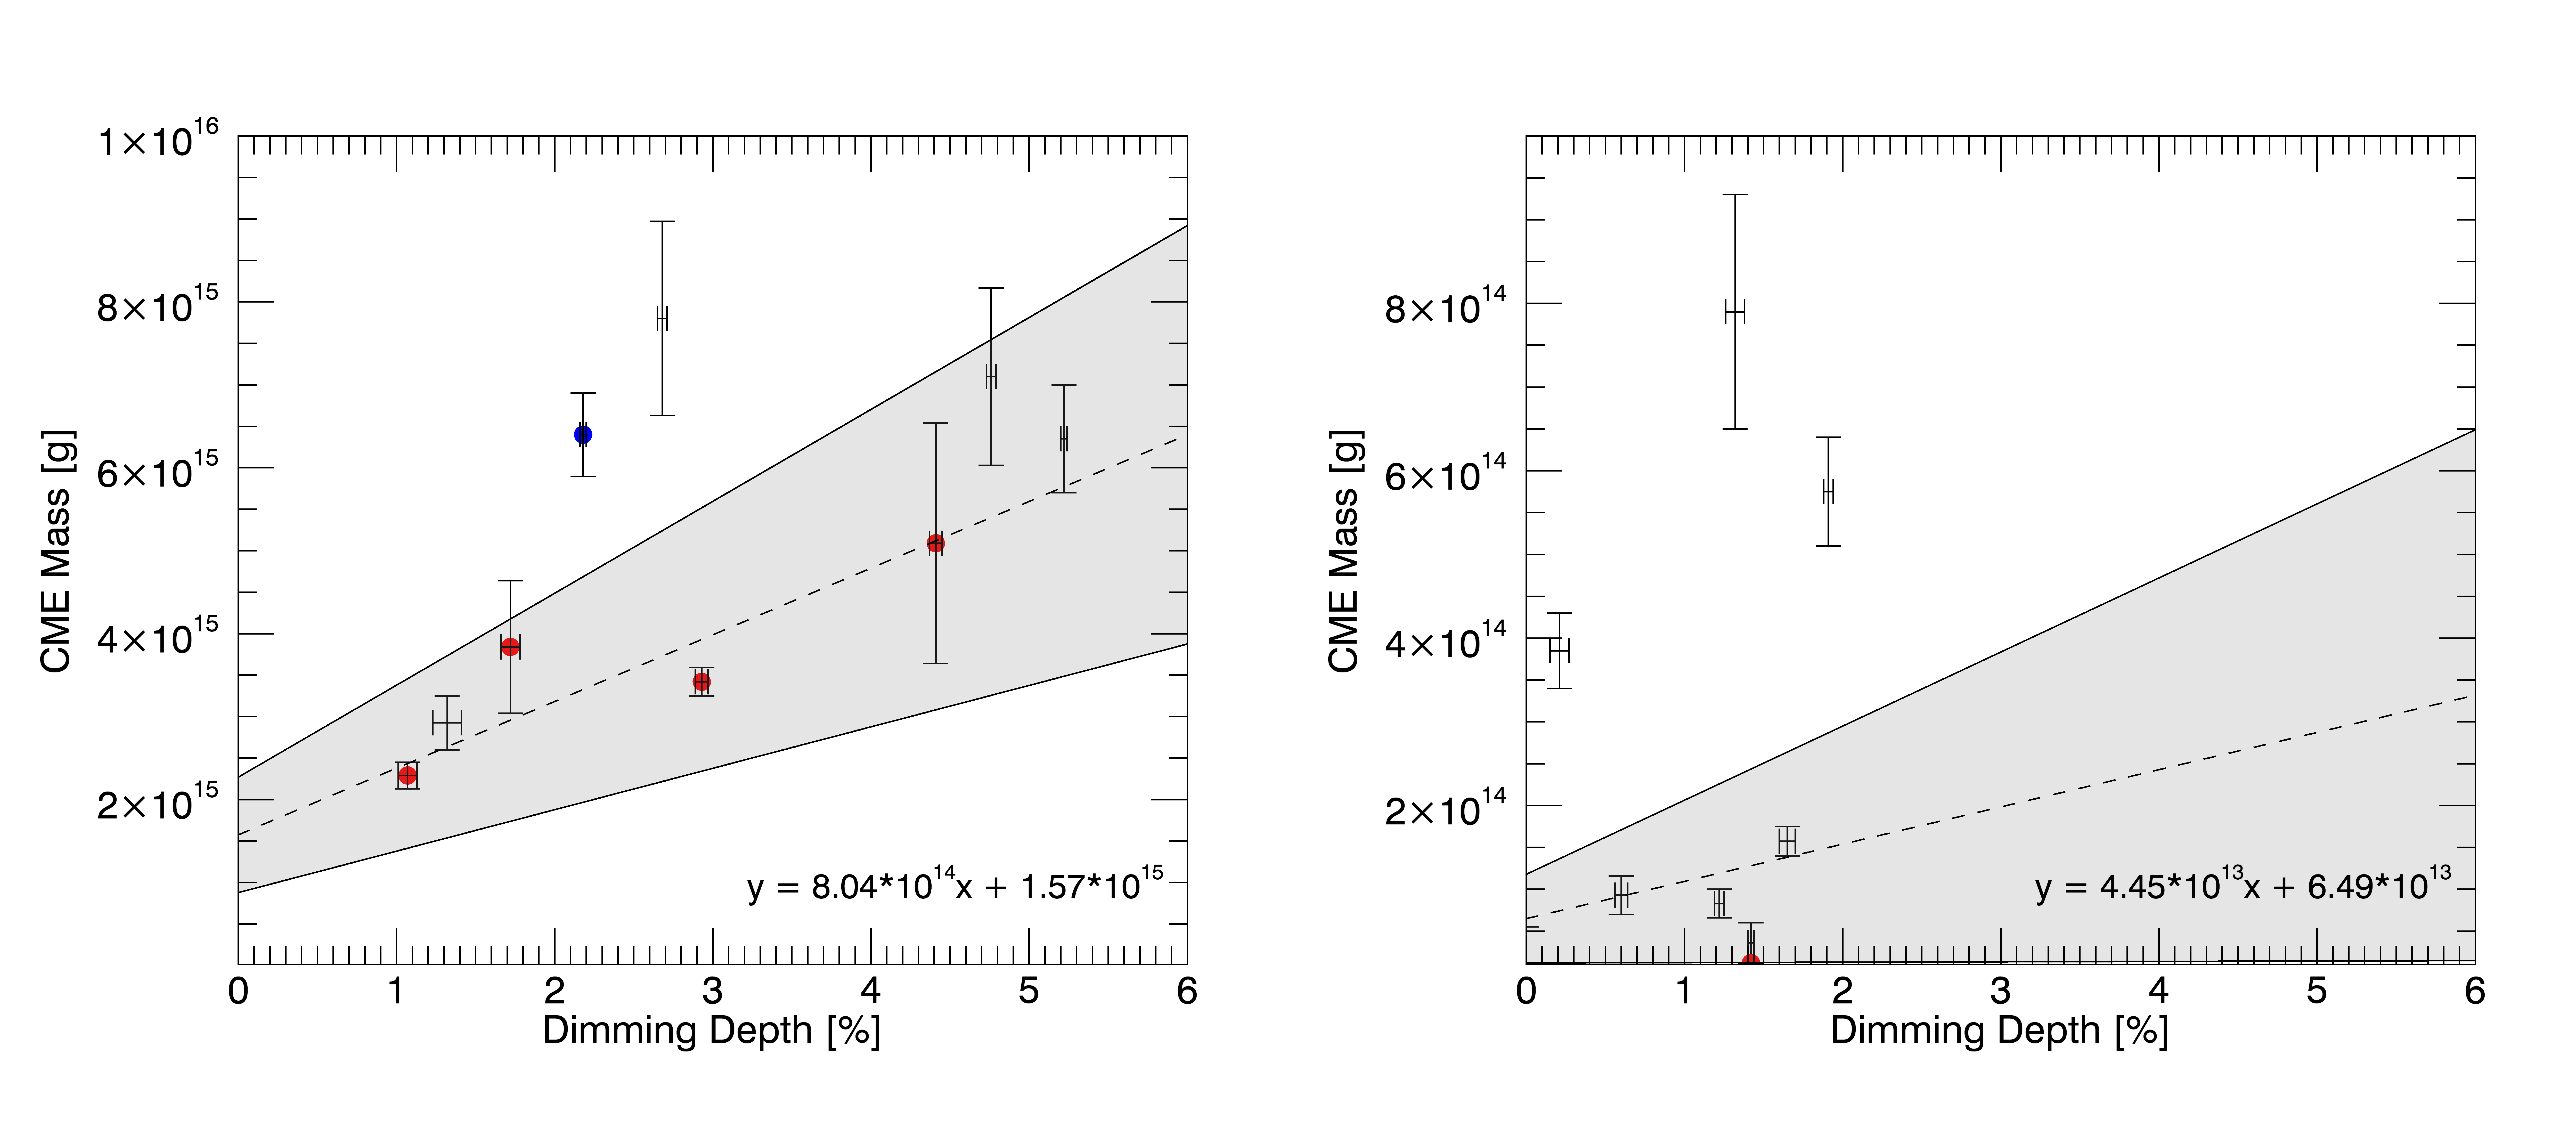
\includegraphics[width=\textwidth]{Images/CorrelationsMassHighAndLow.png}
    \end{center}
    \caption[Correlations: dimming depth vs high and low CME mass]{
        Same as Figure \ref{fig:correlations} but for (left) high CME mass ($\geq\ 1 \times 10^{15}\ g$) and dimming depth 
        and (bottom) low CME mass ($< 1 \times 10^{15} g$) and dimming depth. 
   	}
    \label{fig:correlationshighlowmass}
\end{figure}

The $1\sigma$ uncertainties were computed by \textit{fitexy} for each of these linear fits (note that the shaded regions in Figure \ref{fig:correlations} are $3\sigma$). For all-points CME speed versus dimming slope, the fit slope is $7.54 \times 10^2 \pm 9.45 \times 10^1$ and fit y-intercept is $-3.09 \times 10^2 \pm 5.83 \times 10^1$. Assuming a y-intercept of zero and averaging the black and red slopes in Figure \ref{fig:correlations} left, the best estimate for the linear relationship is that the CME speed is $630\ km\ s^{-1}$ times the dimming slope ($\%\ hour^{-1}$).

For CME mass vs dimming depth, the fit slope is $1.90 \times 10^{14} \pm 3.31 \times 10^{13}$ and fit y-intercept is $8.04 \times 10^{13} \pm 4.15 \times 10^{13}$. Averaging the 3D-derived and high-mass-only slopes, the best estimate for the linear relationship is that the CME mass is $1.03 \times 10^{15} g$ times the dimming depth (\%).

Uncertainties are not factored into the Pearson correlation coefficients quoted in Table \ref{tab:correlations}. Future work could use additional techniques for correlation that account for uncertainty, e.g., rank order. Such a study could include many more events to maximize the efficacy of the correlation comparison.

\section{Summary} 
\label{sec:chapter5summary}
Positive correlations with a high degree of significance have been found between coronal dimming and CME parameters, providing evidence for our initial hypotheses that 1) dimming slope should be directly proportional to CME velocity, and 2) dimming depth should be directly proportional to CME mass. This existence of the correlation was predicted by physical theory. Linear fits between dimming slope and CME speed and between dimming depth and CME mass are provided in Section \ref{sec:correlation}. Additionally, we found that the Fe IX 171 \AA\ dimming corrected for the flare contributions using the Fe XV 284 \AA\ line provides the most accurate dimming results for the EVE data. We note that the uncertainties for coronagraph and dimming parameters are complimentary: there are smaller uncertainties for CME speed than dimming slope, and there are smaller uncertainties for dimming depth than CME mass.